
\documentclass[11pt,a4paper]{article}
\usepackage{jheppub,amsmath, amsthm, amssymb,slashed,url,diagram,bm}
\usepackage{graphicx}
\usepackage{epstopdf}
\usepackage{tcolorbox}
\def\t{\widetilde} 
\def\ct{{\cmmib t}}
\def\btau{{\bm \tau}}
\def\s{{s}}
\def\tr{\mathrm{Tr}}
\def\NSthree{{\mathrm{NS}}^3}
\def\NSRR{{\mathrm{NS}}\cdot{\mathrm{R}}^2}
\def\be{\begin{equation}}
\def\ee{\end{equation}}
\def\bt{{{t}}}
\def\frakn{{\mathfrak N}}
\def\frakl{{\mathfrak L}}
\def\eusmn{{\eusm N}}
\def\Im{{\mathrm{Im}}}
\def\PGL{{\mathrm{PGL}}}
\def\OSp{{\mathrm{OSp}}}
\def\hat{\widehat}
\def\tilde{\widetilde}
\def\frak{\mathfrak}
\def\D{{\mathcal D}}
\def\S{{\mathcal S}}
\def\RP{{\Bbb{RP}}}
\def\NS{{\mathrm{NS}}}
\def\Ra{{\mathrm{R}}}
\def\W{{\mathcal W}}
\def\WW{\mathfrak W}
\def\MM{\mathfrak M}
\def\euq{{\eusm F}}
\def\O{{\mathcal O}}
\def\V{{\mathcal V}}
\def\k{{\cmmib k}}
\def\w{{u}}
\def\dzzt{\D(\t z,z|\theta)}
\def\dzztt{\D(\t z,z|\t\theta,\theta)}
\def\Bbb{\mathbb}
\def\SIgma{\Sigma}
\def\red{{\mathrm{red}}}
\def\A{{\mathcal A}}
\def\d{{\mathrm d}}
\def\tW{{W}}
\def\intt{{\mathrm{int}}}
\def\b{\overlineAn}
\def\R{{\mathbb R}}
\def\RR{{\mathcal R}}
\def\C{{\mathbb C}}
\def\U{{\mathcal U}}
\def\D{{\mathcal D}}
\def\B{{\mathcal B}}
\def\G{{\mathcal G}}
\def\[{\bigl [}
\def\Spin{{\mathrm{Spin}}}
\def\]{\bigr ]}
\def\CP{{\mathbb{CP}}}
\def\N{{\mathcal N}}
\def\T{{\mathcal T}}
\def\p{{'}}
\def\Z{{\mathbb Z}}
\def\Q{{\mathbb Q}}
\def\half{{\frac{1}{2}}}
\def\CC{{\mathcal C}}
\def\ad{{\mathrm{ad}}}
\def\Btriv{{\mathcal B}_{\mathrm{triv}}}
\def\L{{\eusm L}}
\def\h{\hat }
\def\h{\widehat}
\def\Bcc{{\mathcal B_{\mathrm{cc}}}}
\def\K{{\mathcal K}}
\def\V{{\mathcal V}}
\def\J{{\mathcal J}}
\def\I{{\mathcal I}}
\def\P{{\mathcal P}}
\def\B{{\mathcal B}}
\def\Boper{{\mathcal B_{\mathrm{oper}}}}
\def\M{{\mathcal M}}
\def\W{{\mathcal W}}
\def\X{\mathcal X}
\def\Y{\mathcal Y}
\def\P{{\mathcal P}}
\def\l{\langle}
\def\r{\rangle}
\def\H{{\mathcal H}}
\def\ZZ{\eusm B}
\def\cZ{\mathcal Z}
\def\sW{{ W}}
\def\epsilon{\varepsilon}
\def\sY{{ Y}}
\def\nY{{\mathcal Y}}
\def\ca{{\cmmib a}}
\def\ss{{d}}
\def\sf{{\mathfrak s}}
\def\e{{\mathbf e}}
\def\i{{\mathbf i}}
\def\spin{{\mathrm{spin}}}
\def\m{\cmmib m}
\def\tilde{\widetilde}
\def\bar{\overline}
\def\neg{\negthinspace}
\def\Ber{{\mathrm {Ber}}}
\def\BBer{{\text{\it{Ber}}}}
\def\TT{{\mathrm T}}
\def\Tr{{\mathrm {Tr}}}
\def\E{\mathbb{E}}
\def\i{\mathbb{I}}

\font\teneurm=eurm10 \font\seveneurm=eurm7 \font\eighteurm=eurm8 \font\fiveeurm=eurm5
\newfam\eurmfam
\textfont\eurmfam=\teneurm \scriptfont\eurmfam=\seveneurm
\scriptscriptfont\eurmfam=\fiveeurm
\def\eurm#1{{\fam\eurmfam\relax#1}}
%\font\teneurm=eurm10 \font\seveneurm=eurm7 \font\fiveeurm=eurm5
%\newfam\eurmfam
%\textfont\eurmfam=\teneurm \scriptfont\eurmfam=\seveneurm
%\scriptscriptfont\eurmfam=\fiveeurm
%\def\eurm#1{{\fam\eurmfam\relax#1}}
\font\teneusm=eusm10 \font\seveneusm=eusm7 \font\fiveeusm=eusm5
\newfam\eusmfam
\textfont\eusmfam=\teneusm \scriptfont\eusmfam=\seveneusm
\scriptscriptfont\eusmfam=\fiveeusm
\def\eusm#1{{\fam\eusmfam\relax#1}}
\font\tencmmib=cmmib10 \skewchar\tencmmib='177
\font\sevencmmib=cmmib7 \skewchar\sevencmmib='177
\font\fivecmmib=cmmib5 \skewchar\fivecmmib='177
\newfam\cmmibfam
\textfont\cmmibfam=\tencmmib \scriptfont\cmmibfam=\sevencmmib
\scriptscriptfont\cmmibfam=\fivecmmib
\def\cmmib#1{{\fam\cmmibfam\relax#1}}
\def\F{\eusm F}
\def\Pi{\varPi}
\def\g{\text{{\teneurm g}}}
\def\sg{\text{{\eighteurm g}}}
\def\ssg{\text{{\seveneurm g}}}
\def\n{\text{{\teneurm n}}}
\def\sn{\text{{\eighteurm n}}}
\def\ssn{\text{{\seveneurm n}}}
\def\m{\text{{\teneurm m}}}
\def\sm{\text{{\eighteurm m}}}
\def\ssm{\text{{\seveneurm m}}}
\newtheorem{theorem}{Theorem}[subsection]
\newtheorem{lemma}{Lemma}[subsection]
\newtheorem{definition}{Definition}[subsection]
\newtheorem{problem}{Problem}
\newtheorem{algorithm}{Algorithm}[subsection]

\title{Paper Summary}

 \author{Yu Chen}
\affiliation{The Chinese University of HongKong, Department of Mechanical and Automation Engineering}
\emailAdd{anschen@link.cuhk.edu.hk}




\begin{document}\maketitle
%-------------------------------------------------------------------------------------------------------------------------------------------------
\section{Policy Gradient Methods for Reinforcement Learning with Function Approximation}
This article\cite{sutton2000policy} show theoretical possibility of using approximator to encode a policy. In this paper, the author prove the results for both two value functions, one is average reward,
\begin{align}
& V^{\pi}(s) = \lim_{n\to \infty}\frac{1}{n}\E[r_1+r_2+\ldots+r_n|s,\pi] \\ 
& Q^{\pi}(s,a) = \E[\sum_{t=1}^{+\infty}r_t-V^{\pi}(s)|s,a,\pi],
\end{align}
the other is state-by-state reward,
\begin{align}
& V^{\pi}(s) = \E[\sum_{t=1}^{\infty}\gamma^{t-1}r_t|s,\pi],\\
& Q^{\pi}(s,a) = \E[\sum_{k=1}^{\infty}\gamma^{k-1}r_{t+k}|s_t=s,a_t=a,\pi]
\end{align}
We use parameters $\theta$ to approximate policy $\pi$, which means $\pi(s,a) = \pi(s,a;\theta)$.
\begin{theorem}[Policy Gradient]
For any MDP, in either the average-reward or state-state formulatios,
\begin{equation}
\frac{\partial V^{\pi}(s)}{\partial \theta} = \int dsda\rho^{\pi}(s)\frac{\partial \pi(s,a)}{\partial \theta} Q^{\pi}(s,a),
\end{equation}
where $\rho^{\pi}(s)$ is discounted density for state $s$, defined as,
\begin{align}
& \rho^{\pi}(s) = \lim_{t\to\infty}p(s_t|s_0,\pi), \mathrm{stationary \ distribution\ for\ average\ reward}, \\ 
& \rho^{\pi}(s) = \sum_{t=0}^{\infty}\gamma^t p(s_t=s|s_0,\pi), \mathrm{state-state\ formulation}.
\end{align}
\end{theorem}
\emph{Proof}:
\begin{lemma}
The state value function can be written as,
\begin{equation}
V^{\pi}(s) = \int dsda \rho^{\pi}(s)\pi(s,a)R_{s}^{a},
\end{equation}
where $R_{s}^a = \int ds' rp(r,s'|s,a)$, where $p(r,s'|s,a)$ is transition probability of MDPs.
\end{lemma}
Now, we firstly prove average-reward scheme.
\begin{align}
\frac{\partial V^{\pi}(s)}{\partial \theta} & = \frac{\partial}{\partial \theta}\sum_a \pi(s,a)Q^{\pi}(s,a) \\ 
& = \sum_a \partial_{\theta}\pi Q^{\pi} + \pi \partial_{\theta}Q^{\pi} \\ 
& = \sum_a \partial_{\theta}\pi Q^{\pi} + \pi \partial_{\theta}\left(R_{s}^a - V^{\pi}(s)+\sum_{s'}p(s'|s,a)V^{\pi}(s')\right)\\ 
& = \sum_{a}\left(\partial_{\theta}\pi Q^{\pi} + \pi\sum_{s'}p(s'|s,a)\partial_{\theta}V^{\pi}(s')\right) - \partial_{\theta}V^{\pi}(s).
\end{align}
Since, for averaged reward, the value function depends on the final stationary distribution, we can,
\begin{equation}
\aligned
\sum_{s}\rho^{\pi}(s)\partial_{\theta}V^{\pi}(s) = &\sum_{s,a}\rho^{\pi}(s)Q^{\pi}(s,a)\partial_{\theta}\pi(s,a) + \sum_{s,a,s'}p(s'|s,a)\pi(s,a)\rho^{\pi}(s)\partial_{\theta}V^{\pi}(s')\\ & - \sum_{s}\rho^{\pi}(s)\partial_{\theta}V^{\pi}(s)\\ 
= & \sum_{s,a}\rho^{\pi}(s)Q^{\pi}(s,a)\partial_{\theta}\pi(s,a) + \sum_{s'}\rho^{\pi}(s')\partial_{\theta}V^{\pi}(s') - \sum_{s}\rho^{\pi}(s)\partial_{\theta} V^{\pi}(s)\\ 
= & \sum_{s,a}\rho^{\pi}(s)Q^{\pi}(s,a)\partial_{\theta}\pi(s,a).
\endaligned
\end{equation}
QED.\\ 
For state-state formulation, we can compute as,
\begin{align}
\partial_{\theta}V^{\pi}(s) & = \sum_{a}\partial_{\theta}\pi Q^{\pi} + \pi \partial_{\theta}Q^\pi \\ 
& = \sum_a \partial_{\theta}\pi Q^{\pi} + \pi \partial_{\theta}\sum_{s'}rp(r,s'|s,a)+\gamma p(s'|s,a)V^{\pi}(s')\\ 
& = \sum_a \partial_{\theta}\pi(s,a) Q^{\pi}(s,a) + \pi(s,a) \gamma p(s'|s,a)\partial_{\theta}V^{\pi}(s') \\ 
& \ddots \\ 
& = \sum_{s}\rho^{\pi}(s)\sum_{a}Q^{\pi}(s,a)\partial_{\theta}\pi(s,a).
\end{align}
From the above, we can find gradient of policy depends only on $Q^{\pi}(s,a)$ and is independent of $\partial_{\theta}Q^{\pi}$, which brings greate convinience. Then, we can introduce another approximation with parameters $\omega$ to approximate $Q$ value function, denoted by $f_{w}(s,a)$. To make $f_w \to Q$, the following equation should be satisfied,
\begin{equation}
\aligned 
& \partial_w \sum_{s}\sum_{a}\rho^\pi(s,a)\pi(s,a)(Q(s,a)-f_w(s,a))^2 = 0 \\ 
\label{eq:approx_q}
& \Leftrightarrow \sum_{s}\sum_{a}\rho^\pi(s,a)\pi(s,a)(Q(s,a)-f_w(s,a))\partial_w f_w(s,a) = 0.
\endaligned
\end{equation}
\begin{theorem}[Policy Gradient with Function Approximation]
If $f_{\omega}$ satisfies Eq.(\ref{eq:approx_q}) and,
\begin{equation}
\label{eq: cons}
\frac{\partial f_w(s,a)}{\partial \omega} = \frac{\partial \pi(s,a)}{\partial \theta}\frac{1}{\pi(s,a)},
\end{equation}
then,
\begin{equation}
\frac{\partial V^{\pi}(s)}{\partial \theta} = \sum_{s}\rho^{s}(\pi)\sum_{a}\frac{\partial \pi(s,a)}{\partial \theta}f_w(s,a).
\end{equation}
\end{theorem}
The proof is obivous. In the following, we can discuss Eq.(\ref{eq: cons}), and construct approximators satisfying it. For example, we use a Gibbs distribution to parameterize $\pi(s,a)$ as,
\begin{equation}
\pi(s,a;\theta) = \frac{e^{\theta^T \phi(s,a)}}{\sum_{a'}e^{\theta^T\phi(s,b)}}.
\end{equation}
And then, we obtain,
\begin{equation}
\frac{1}{\pi(s,a)}\frac{\partial \pi(s,a)}{\partial \theta} = \phi(s,a) - \sum_{b}\pi(s,b)\phi(s,b)
\end{equation}
Hence, we just need to parameterize $f_w(s,a)$ as,
\begin{equation}
f_w(s,a) = w^T(\phi(s,a)-\sum_b \pi(s,b)\phi(s,b)).
\end{equation}

\begin{theorem}[Policy Iteration with Function Approxmimation]
Let $\pi$ and $f_w$ be any differential function approximators for the policy and value function respectively that satisfy the compatibility condition\ref{eq: cons} and for which $\max_{\theta,s,a,i,j}|\frac{\partial^2\pi(s,a)}{\partial\theta_I\partial\theta_j}|<B<\infty$. Let $\{\alpha_k\}_{k=0}^{+\infty}$ be any step-size sequence such that $\lim_{k\to\infty} \alpha_k =0$ and $\sum_k \alpha_k = \infty$. Then for any MDP with bounded rewards, the sequence $\{V^{\pi_k}\}$, defined by any $\theta_0, \pi_k$, and,
\begin{align}
& w_k = w\ \mathrm{such\ that}\ \sum_{s}\rho^{\pi_k}\sum_a\pi_k(s,a)(Q^{\pi_k}(s,a)-f_w(s,a))\partial_w f_w(s,a) = 0, \\ 
& \theta_{k+1} = \theta + \alpha_k \sum_{s}\rho^{\pi_k}(s)\sum_af_{w_k}(s,a)\partial_{\theta}\pi_k(s,a),
\end{align}
converges such that $\lim_{k\to \infty}\frac{\partial V^{\pi_k}(s)}{\partial \theta} = 0$
\end{theorem}

%-------------------------------------------------------

\section{GTD--gradient temporal difference}
\subsection{ Policy gradient methods for reinforcement learning with function approximation}
The article\cite{NIPS2008_3626} firstly raises idea for off-policy gradient temporal difference with a linear function approximator. We denote the stationary distribution of behavior policy $b$ as $\rho^{b}(s)$. The observation of state $s$ is given by $\phi_s \in \mathbb{R}^n$, so the $\delta_t$ is,
\begin{equation}
\delta_t = r_{t} + \gamma V_t(s_{t+1}) - V_t(s_t) = r_t + \gamma \theta^T\phi_{t+1} -\theta^T \phi_t.
\end{equation}
Intutively, we wish the $\delta_t$ approaches to $0$, when we reach a local minimum or maximum. In other words, we can define our obejective function as $L2$ norm,
\begin{equation}
J(\theta) = \E[\delta \phi]^T \E[\delta \phi],
\end{equation}
where $\E$ is over the stationary distribution $\rho^b(s)$. The gradient is,
\begin{align}
\nabla_{\theta}J(\theta)& = 2 \nabla_{\theta}\E[\delta \phi^T] \E[\delta \phi] \\ 
& = -2\E[(\phi-\gamma\phi')\phi^T]\E[\delta\phi].
\end{align}
where $\phi' = \phi_{t+1}$. Hence, there are two approaches two find this gradient. Firstly, it stores the expectation of the first term and samples the second term; secondly, it stores the expectation of the second term and samples the first term. (Note: why we do not stores both expectation is that it will introduce bias brought by the correlation of these two terms). Mathematically, we have $\phi_1,r_1,\phi_2,r_2,\cdots, \phi_k, r_k,\phi_{k+1},r_{k+1}$,
\begin{align}
& A_k = \frac{1}{k}\sum_{j=1}^k(\phi_j-\gamma\phi_{j+1})\phi_j^T, \\ 
& \theta_{k+1} = \theta_k + \alpha_k A_k \delta_k\phi_k,
\end{align}
where $\delta_k = r_k + \gamma \theta_k^T\phi_{k+1}-\theta_k^T\phi_k$. The disadvantage of this method is that finding $A_k \in \mathbb{R}^{n\times n}$ costs our $n^2$ complexity. Hence, the most case we use the second approach,
\begin{align}
& w_{k+1} = w_k + \beta_k (\delta_k\phi_k - w_k), \\ 
& \theta_{k+1} = \theta_k + \alpha_k(\phi_k-\gamma\phi_{k+1})\phi_k^T w_k
\end{align}
\subsection{Fast Gradient-Descent Methods for Temporal-Difference Learning with Linear Function Approximation}
This article \cite{sutton2009fast} give an improvement of the above algorithm, named GTD2 and TDC(TD with gradient correction). GTD2 uses a different obejcetive function,
\begin{equation}
J(\theta) = \E[\delta \phi]^T \E[\phi \phi^T]^{-1} \E[\delta\phi].
\end{equation}
The idea of this objective function comes from the following facts. The ultimate goal of these algorithm is to find an approximator $V_{\theta}$, which can approximates $V$ as exactly as possible. As we known, the true $V$ satisfies the Bellman equation,
\begin{equation}
V = TV,
\end{equation}
where $T$ is Bellman transition matrix. Hence, we hope our approximator can satisfies this property too, in other wrods, we wish $\|V_{\theta}-TV_{\theta}\|^2_{\rho^b} \equiv \int ds \rho^b(s)|V_{\theta}(s)-TV_{\theta}(s)|^2 \to 0$. Unfornuately, $TV_{\theta}$ may not stay in the space $V_{\theta}$. Instead, we denote a projector $\Pi$, which projects any $v$ to space $V_{\theta}$ as $\Pi v$. To find $\Pi$, we firstly find $\theta$ minimizing $\|v-\Phi\theta\|_D$, where $D \in \mathbb{R}^{|\mathcal{S}|\times |\mathcal{S}|}$ is diagonal matrix with element $\rho^{b}(s)$, and $\Phi$ with rows $\phi_s$.
\begin{equation}
\nabla_{\theta} \|v - \Phi\theta\|_D^2 = -2\Phi^TD(v-\Phi\theta),
\end{equation}
which means $\theta = (\Phi^TD\Phi)^{-1}\Phi^TDv$, and we know $\Pi v=\Phi\theta, \forall v$. Hence,
\begin{equation}
\Pi = \Phi(\Phi^TD\Phi)^{-1}\Phi^TD
\end{equation}
We define mean-squared projected Bellman error as,
\begin{equation}
\mathrm{MSPBE}(\theta) \equiv \|V_{\theta}-\Pi TV_{\theta}\|^2_D.
\end{equation}
By using the facts,
\begin{equation}
\aligned 
&\E[\phi \phi^T] = \sum_s d_s\phi_s\phi_s^T = \Phi^T D \Phi,\\
& \E[\delta\phi] = \sum_s d_s\phi_s(R_s+\gamma \sum_{s'}p_{s,s'}V_{\theta}(s')-V_{\theta}(s)) = \Phi^T D (TV_{\theta} - V_{\theta}), \\ 
& \Pi^T D \Pi = D^T \Phi(\Phi^T D \Phi)^{-1} \Phi^T D.
\endaligned 
\end{equation}
we can simplify $\mathrm{MSPBE}(\theta)$ as
\begin{equation}
\aligned 
\mathrm{MSPBE}(\theta) & = \|V_{\theta}-\Pi T V_{\theta}\|_D^2 \\ & = (V_{\theta} -\Pi T V_{\theta})^T D (V_{\theta} -\Pi T V_{\theta}) \\ & = (V_{\theta}-TV_{\theta})^T\Pi^TD\Pi(V_{\theta}-TV_{\theta}) \\ & = (V_{\theta}-TV_{\theta})^TD^T \Phi(\Phi^T D \Phi)^{-1} \Phi^T D(V_{\theta}-TV_{\theta}) \\ 
& = \E[\delta \phi]^T \E[\phi\phi^T]^{-1} \E[\delta\phi].
\endaligned 
\end{equation}
The gradient is,
\begin{equation}
\nabla_{\theta}\mathrm{MSPBE}(\theta) = -2\E[(\phi-\gamma\phi')\phi^T]\E[\phi\phi^T]^{-1}\E[\delta\phi].
\end{equation}
We use $w$ to approximate $\E[\phi\phi^T]^{-1}\E[\delta\phi]$, so the update rule is,
\begin{align}
& w_{k+1} = w_k + \beta_k(\delta_k - \phi_k^Tw_k)\phi_k, \\ 
& \theta_{k+1} = \theta_k + \alpha_k(\phi_k-\gamma\phi_k')(\phi_k^Tw_k).
\end{align}
TDC apprixmates this gradient more exactly,
\begin{align}
-\frac{1}{2}\nabla_{\theta}\mathrm{MSPBE}(\theta) & =\E[(\phi-\gamma\phi')\phi^T]\E[\phi\phi^T]^{-1}\E[\delta\phi] \\ 
& = \E[\delta\phi]-\gamma \E[\phi'\phi^T]\E[\phi\phi^T]^{-1}\E[\delta\phi] \\ 
& \approx  \E[\delta\phi] - \gamma \E[\phi'\phi^T]w
\end{align}
Hence, TDC update $\theta$ as,
\begin{equation}
\theta_{k+1} = \theta_k + \alpha_k\delta_k\phi_k - \alpha \gamma \phi_k'(\phi_k^Tw_k).
\end{equation}

\begin{tcolorbox}[title=Gradient Temporal Diffierence]
\begin{align}
& w_{k+1} = w_k + \beta_k(\delta_k - \phi_k^Tw_k)\phi_k, \\ 
& \theta_{k+1} = \theta_k + \alpha_k(\phi_k-\gamma\phi_k')(\phi_k^Tw_k)\quad \textbf{(GTD2)}, \\ 
& \theta_{k+1} = \theta_k + \alpha_k\delta_k\phi_k - \alpha \gamma \phi_k'(\phi_k^Tw_k) \quad \textbf{(TDC)}.
\end{align}
\end{tcolorbox}

\subsection{GTD$(\lambda)$}
Above two algorithms are about GTD$(0)$, in these section, the author introduce the final version of GTD--GTD$(\lambda)$\cite{maei2011gradient}. Firstly, we can write $\lambda-$return as,
\begin{equation}
G_t^{\lambda} = r_{t+1} + \gamma\left((1-\lambda)V(s_{t+1})+\lambda G_{t+1}^{\lambda}\right).
\end{equation}
Obviously, when $\lambda=1$ it is MC method, $\lambda=0$ is dynamical programming. For simiplicity, we also use linear approximation, so the $\delta$ return is,
\begin{align}
& G_t^\lambda = r_{t+1} + \gamma(1-\lambda) \theta^T\phi_{t+1} + \gamma \lambda G_{t+1}^{\lambda},\\
& \delta_t^{\lambda} = G_{t}^\lambda - \theta^T\phi_t
\end{align}
Similarly, we can define a new operator as,
\begin{equation}
\P_{b}^{\pi}\delta_t^{\lambda}\phi_t := \sum_s \rho^b(s)\E[\delta_t^\lambda|S_t=s,\pi]\phi(s)
\end{equation}
We can find it has the following properties,
\begin{equation}
\E[\delta_t^\lambda|S_t=s,\pi] = \E[G_{t}^{\lambda}-\theta^T\phi_s|S_t=s,\pi] = TV_{\theta}(s) - V_{\theta}(s)
\end{equation}
then,
\begin{align}
\P_{b}^{\pi}\delta_t^{\lambda}\phi_t &= \sum_s \rho^b(s)\E[\delta_t^\lambda|S_t=s,\pi]\phi(s)\\ 
& = \sum_s \rho^b(s)(TV_{\theta}(s)-V_{\theta}(s))\phi(s) \\ 
& = \Phi^T D (TV_{\theta}-V_{\theta}).
\end{align}
Hence,
\begin{equation}
\mathrm{MSPBE}(\theta) = \|V_{\theta} - \Pi TV_{\theta}\|_D^2 = (\P_{b}^{\pi}\delta_t^\lambda \phi_t)^T \E[\phi_t\phi_t^T]^{-1}\P_{b}^{\pi}\delta_t^\lambda \phi_t.
\end{equation}
Here there is a problem $\P_{b}^{\pi}\delta_t^\lambda \phi_t$ is along trajectory by $\pi$, but our sample is along $b$. Hence we need to use importance sampling to solve it. To this end, we define,
\begin{align}
& G_{t}^{\lambda\rho}(\theta) = \rho_t(r_{t+1}+\gamma((1-\lambda)\theta^T\phi_t + \lambda G_{t}^{\lambda\rho}(\theta))),\\ 
& \delta_{t}^{\lambda \rho}(\theta) = G_t^{\lambda \rho}(\theta) - \theta^T\phi_t.
\end{align}
where $\rho_t = \frac{\pi(S,A)}{b(S,A)}$.
\begin{theorem}[Off-policy with importance sampling]
\begin{equation}
\P_{b}^{\pi}\delta_t^\lambda(\theta) \phi_t = \E[\delta_t^{\lambda\rho}(\theta)\phi_t].
\end{equation}
\end{theorem}
\emph{Proof}:
To prove this, we only need to prove the following,
\begin{equation}
\E[G_t^{\lambda\rho}\phi_t|S_t=s] = \E[G_t^{\lambda}\phi_t|S_t=s,\pi].
\end{equation}
We compute the left side,
\begin{equation}
\aligned 
\E[G_t^{\lambda\rho}|S_t=s]  =& \E[\rho_t R_{t+1} + \rho_t\gamma(1-\lambda)\theta^T\phi_t|S_t=s] + \gamma\lambda \E[\rho_tG_{t+1}^{\lambda\rho}|S_t=s] \\ 
 =& \E[R_{t+1}+\gamma(1-\lambda)\theta^T\phi_t|S_t=s,\pi] + \\
 & + \gamma\lambda\sum_{s'}p(s'|s,a)b(s,a)\frac{\pi(s,a)}{b(s,a)}\E[G_{t+1}^{\lambda}|S_{t+1}=s'] \\ 
 = & \E[R_{t+1}+\gamma(1-\lambda)\theta^T\phi_t|S_t=s,\pi] + \lambda \gamma \E[G_{t+1}^{\lambda}|S_t=s,\pi] \\ 
 = & \E[G_{t}^\lambda|S_t=s,\pi].
\endaligned 
\end{equation}
Hence,
\begin{equation}
\mathrm{MSPBE}(\theta) = \E[\delta_t^{\lambda\rho}\phi_t]^T\E[\phi_t\phi_t^T]^{-1}\E[\delta_t^{\lambda\rho}\phi_t].
\end{equation}
This is forward view, to implement this algorithm, we need to find $e_t$ such that $\E[\delta_t^{\lambda\rho} \phi_t] = \E[\delta_t e_t]$, where $\delta_t$ is common TD difference $\delta_t = r_{t+1} + \gamma \theta^T\phi_{t+1}-\theta^T\phi_t$.
\begin{theorem}[Equivalence of the TD forward-view and backward-view] The forward-view is equivalent to the following backward-view:
\begin{equation}
\E[\delta_t^{\lambda\rho} \phi_t] = \E[\delta_t e_t]
\end{equation}
with updating rule,
\begin{equation}
e_t = \rho_t (\phi_t + \gamma\lambda e_{t-1}).
\end{equation}
\end{theorem}
\emph{Proof}:
We simplify $\delta_t^{\lambda\rho} = G_{t}^{\lambda\rho}-\theta^T\phi_t$ step by step.
\begin{align}
G_{t}^{\lambda\rho} & = \rho_t(r_{t+1}+\gamma \theta^T\phi_{t+1}-\theta^T\phi_t)+\rho_t\theta^T\phi_t - \lambda\gamma\rho_t\theta^T\phi_{t+1}+\lambda\gamma\rho_tG_{t+1}^{\lambda\rho} \\ 
& = \rho_t\delta_t(\theta)+\rho_t\theta^T\phi_t+\lambda\gamma\rho_t\delta_{t+1}^{\lambda\rho}. 
\end{align}
Hence,
\begin{equation}
\delta_t^{\lambda\rho} = \rho_t\delta_t + (\rho_t-1)\theta^T\phi_t + \lambda\gamma\rho_t\delta_{t+1}^{\lambda\rho}.
\end{equation}
We firstly prove the second term vanishes under expectation,
\begin{align}
\E[(1-\rho_t)\theta^T\phi_t\phi_t] & = \sum_{s,a} b(s,a)\rho^b(s)(1-\frac{\pi(s,a)}{b(s,a)})\theta^T\phi_s\phi_s \\ 
& = \sum_{s,a} \rho^b(s)(b(s,a)-\pi(s,a))\theta^T\phi_s\phi_s \\ & = \sum_s \rho^b(s)(1-1)\theta^T\phi_s\phi_s = 0. 
\end{align}
Hence,
\begin{equation}
\aligned
 \E[\delta_t^{\lambda\rho}\phi_t] &= \E[\rho_t\delta_t\phi_t + \lambda\gamma\rho_t\delta_{t+1}^{\lambda\rho}\phi_t] \\ 
& = \E[\rho_t\delta_t\phi_t] + \lambda\gamma\E[\rho_{t-1}\delta_{t}^{\lambda\rho}\phi_{t-1}] \\ 
& = \E[\rho_t\delta_t\phi_t + \lambda\gamma \rho_{t-1}\phi_{t-1}\rho_t\phi_t] + \gamma^2\lambda^2\E[\rho_{t-1}\rho_t\delta_{t+1}^{\lambda\rho}\phi_{t-1}\phi_t] \\ 
& \ddots \\ 
& = \E[\delta_t\rho_t(\phi_t+\lambda\gamma\phi_{t-1}\rho_{t-1}+\cdots)]\\ 
& = \E[\delta_t e_t],
\endaligned 
\end{equation}
with $e_t = \rho_t(\phi_t + \gamma\lambda e_{t-1})$.\\ 
Now, we can find gradient of $\mathrm{MSPBE}(\theta) = \E[\delta_te_t]^T\E[\phi_t\phi_t^T]^{-1}\E[\delta_te_t]$.
\begin{equation}
-\frac{1}{2}\nabla_{\theta}\mathrm{MSPBE}(\theta) = -\E[\gamma(\phi_{t+1}-\phi_t)e_t^T]\E[\phi_t\phi_t^T]^{-1}\E[\delta_te_t].
\end{equation}
To simplify it, we use the following equalities,
\begin{equation}
\aligned
\E[\phi_t\rho_t\phi_t^T] = \E[\phi_t\phi_t^T], \E[\phi_{t+1}\rho_te_t^T] = \E[\phi_{t+1}e_t^T]
\endaligned 
\end{equation}
\begin{align}
\E[\phi_t e_t^T] & = \E[\phi_t\rho_t(\phi_t^T+\lambda\gamma e_{t-1}^T)] \\ 
& = \E[\phi_t\phi_t^T] + \gamma\lambda\E[\phi_{t+1}e_t^T].
\end{align}
\begin{equation}
\aligned 
-\frac{1}{2}\nabla_{\theta}\mathrm{MSPBE}(\theta) & = \E[\delta_t e_t] - \gamma(1-\lambda)\E[\phi_{t+1}e_t^T]\E[\phi_t\phi_t^T]^{-1}\E[\delta_te_t] \\ 
& \approx \E[\delta_t e_t] - \gamma(1-\lambda)\E[\phi_{t+1}e_t^T]w.
\endaligned
\end{equation}
Hence updating rule is,
\begin{align}
& \theta_{t+1} = \theta_t + \alpha_t(\delta_t e_t - \gamma(1-\lambda)(e_t^T w_t)\phi_{t+1}), \\ 
& w_{t+1} = w_t + \beta_t (\delta_t e_t -(w_t^T\phi_t)\phi_t),\\ 
& e_{t+1} = \rho_t(\phi_t + \gamma \lambda e_{t-1}).
\end{align}
\begin{tcolorbox}[title=GTD$(\lambda)$ with linear function approximation]
Initialize $w_0$ to $0$, and $\theta_0$ arbitarily. \par 
Choose $\alpha,\beta,\gamma,\lambda$ \par 
Reapeat for each episode:\par 
\hspace{1cm} Initilize $e=0$ \par 
\hspace{1cm} Take $A_t$ from $S_t$ according to $b(a|s)$ and observe $(\phi_t,r_{t+1},\phi_{t+1})$ \par 
\hspace{1cm} Update as:
\hspace{1cm} 
\begin{equation*}
\aligned 
& \delta_t \leftarrow r_{t+1} + \gamma \theta^T \phi_{t+1} - \theta^T\phi_t. \\ 
& \rho_t \leftarrow \frac{\pi(a_t|s_t)}{b(a_t|s_t)} \\ 
& e_t \leftarrow \rho_t (\phi_t + \lambda\gamma e_{t-1}) \\ 
& \theta_{t+1} \leftarrow \theta_t + \alpha_t[\delta_t e_t -\gamma(1-\lambda)(e_t^Tw_t)\phi_{t+1}] \\ 
& w_{t+1} \leftarrow w_t + \beta_t(\delta_t e_t - (\phi_t^T w_t)\phi_t).
\endaligned
\end{equation*}
\end{tcolorbox}
%-------------------------------------------------------------

\section{Off Policy Actor-Critic}
This article\cite{degris2012off} introduce the first actor-critic method that can be applied off-policy, give off-policy gradient theorem and convergence proof. In this paper, author use $b$ to denote the behaviour policy, and stationary distribution or discounted distribution is $\rho^{b}(s)$ in our notations. The objective function is,
\begin{equation}
J(\pi_{\theta}) = \int \d s \rho^b(s)V^{\pi_\theta}(s).
\end{equation}
Obviously, we should updata $\theta$ along the direction $\nabla_{\theta}J(\pi_{\theta})$, which is given by,
\begin{equation}
\aligned 
\nabla_{\theta} J(\pi_{\theta}) & = \int \d s \d a \rho^b(s) \nabla_{\theta}(\pi_{\theta}(s,a)Q^{\pi_{\theta}}(s,a)) \\ 
& = \int \d s\d a \rho^b(s)\left(\nabla \pi_{\theta}Q + \pi_{\theta}\nabla_{\theta}Q\right) \\ 
& \equiv g(\theta) + \int \d s \d a \rho^b(s)\pi_{\theta}\nabla_\theta Q.
\endaligned 
\end{equation}
Actually, the second term is very difficult to compute, the following theorem proves that ignoring it is good approximation.
\begin{theorem}[Policy Improvement]
Given any policy with parameters $\theta$, let,
\begin{equation}
\theta' = \theta + \alpha g(\theta).
\end{equation}
Then there exists an $\epsilon > 0$ such that, for all possible $\alpha < \epsilon$,
\begin{equation}
J(\pi_{\theta'}) > J(\pi_{\theta}).
\end{equation}
Further, if $\pi$ has a tabular representation, then
\begin{equation}
 V^{\pi_{\theta'}}(s) > V^{\pi_{\theta}}(s), \forall s.
 \end{equation} 
\end{theorem}
\emph{Proof}:
It is easy to show,
\begin{equation}
\aligned 
J(\pi_{\theta}) & = \int \d s\d a\rho^{b}(s)\pi_{\theta}(s,a)Q^{\pi_{\theta}}(s,a) \\
& \le \int \d s \d a \rho^{b}(s)\pi_{\theta'}(s,a)Q^{\pi_{\theta}}(s,a). 
\endaligned 
\end{equation}
Since we have $f(x+\alpha \nabla f) - f(x) = \alpha (\nabla f)^2 > 0$. Then we repeat applying the above inequality, we can find,
\begin{align}
J(\pi_{\theta}) & \le \E_{s\sim \rho^b, a\sim \pi_{\theta'}}Q^{\pi_{\theta}}(s,a) \\ 
& = \E_{s\sim \rho^b}\E_{a\sim \pi_{\theta'}} [r_{t+1} + \gamma V^{\pi_{\theta}}(s_{t+1})] \\ 
& \le \E_{s\sim \rho^b}\E_{a\sim \pi_{\theta'}}[r_{t+1}+\gamma r_{t+2}+\gamma V^{\pi_{\theta}(s_{t+2})}] \\ 
& \ddots \\ 
& = J(\pi_{\theta'}).
\end{align}
The second part is similar since
\begin{equation}
V^{\pi_{\theta}} = \int \d a \pi_{\theta}(s,a)Q^{\pi_{\theta}}(s,a) \le \int \d a \pi_{\theta'}(s,a)Q^{\pi}(s,a).
\end{equation}
By repeating the above formula, we can prove the second part.
\begin{theorem}[Off Policy Gradient Theorem]
Let $\Z = \{\theta|\nabla_{\theta}J(\pi_{\theta})=0\}$ and $\tilde{\Z}=\{\theta|g(\theta)=0\}$, which are both non-empty by some assumptions. If the value function can be represented by our function class, then,
\begin{equation}
\Z \in \tilde{\Z}.
\end{equation}
Moreover, if we use a tabular representation for policy $\pi$, then
\begin{equation}
\Z = \tilde{\Z}.
\end{equation}
\end{theorem}
\emph{Proof}:
This first part is very trivial because of off policy improvement theorem. More specificly, any $\theta^*$ such that $\nabla_{\theta}J(\pi_{\theta})|_{\theta^*}=0$ must means $g(\theta^*) =0$, otherwise there exists a direction $\frac{g(\theta^*)}{\|g(\theta^*)\|}$ such that $J(\theta)$ increases, which is contradict to $\nabla_{\theta} J(\theta)|_{\theta^*}=0$.\\ 
For the second part, we have a tabular representation, which means each weight corresponds to exactly one state. Without loss of generality, weights $\theta_{s,1},\theta_{s,2},\ldots,\theta_{s,s_n}$ are relative to state $s$. Since $g(\theta^*) = 0$,
\begin{equation}
\label{eq:tabular1}
\int \d s' \d a \rho^b(s)\partial_{\theta_{s,j}}\pi_{\theta}(s',a) Q^{\pi_{\theta}}(s',a)= \rho^{b}(s)\partial_{\theta_{s,j}}\pi_{\theta}(s,a) Q^{\pi_{\theta}}(s,a) = 0, \forall j=1,\ldots,s_n.
\end{equation}
If there exists $k$ such that,
\begin{equation}
\int \d s'\d a \pi_{\theta}(s',a)\partial_{\theta_{s,k}}Q^{\pi_{\theta}}(s',a) \neq 0,
\end{equation}
which means $J(\pi_{\theta})$ will increase for local increasement of $Q^{\pi_{\theta}}(s,a)$. In other words, we can change our policy a litte to increase our objective function, which means,
\begin{equation}
\sum_{j=1}^{n_s}\int \d s' \d a \partial_{\theta_{s,j}}\pi_{\theta}(s',a) Q^{\pi_{\theta}}(s',a) \neq 0.
\end{equation}
Contracted to Eq.(\ref{eq:tabular1}). \\ 
Then, we can rewrite $g(\theta)$ as,
\begin{align}
g(\theta) & = \int \d s \rho^b(s) Q^{\pi_{\theta}}(s,a)\nabla_{\theta}\pi_{\theta}(a|s) \\ 
& = \int \d s \rho^b(s)b(a|s)\rho(a|s)Q^{\pi_{\theta}}(s,a)\nabla \log \pi_{\theta}(a|s) \\ 
& = \E[\rho(s,a)\psi(s,a)Q^{\pi_{\theta}}(s,a)].
\end{align}
There is a famous result that an arbitrary function of state can be introduced into these equations as a baseline without changing the expected value. Hence, we can write $g(\theta)$ as,
\begin{equation}
g(\theta) = \E[\rho(s,a)\psi(s,a)(Q^{\pi}(s,a)-V(s))] \approx \E[\rho(s,a)\psi(s,a)(R_t^{\lambda}-V(s))].
\end{equation}
where $R_t^\lambda$ is off-policy $\lambda-$return, defined as,
\begin{equation}
R_t^\lambda = r_{t+1} + \gamma (1-\lambda)V(s_{t+1}) + \gamma \lambda \rho_t R_{t+1}^\lambda 
\end{equation}
To find a backward-view implement, we need to find $e_t$ such that,
\begin{equation}
\E[\rho(s,a)\psi(s,a)(R_t^{\lambda}-V(s))] = \E[\delta_t e_t],
\end{equation}
where $\delta_t = r_{t+1} + \gamma V(s_{t+1}) - V(s_t)$. As shown in paper, updating rule of $e_t$ is given by,
\begin{equation}
e_t = \rho_t(\psi_t+\lambda\gamma e_{t-1}).
\end{equation}
\begin{tcolorbox}[title=Off-PAC algorithm]
Initialize the vectors $e_v,e_u$ and $w$ to zero\par 
Initialize the vectors $v, u$ arbitrarily \par 
Initialize the state $s$ \par 
For each step: \par 
\hspace{1cm} Choose an action $a$, according to $b(a|s)$ \par 
\hspace{1cm} Observer resultant reward $r$, and next state $s'$, \par 
\begin{equation*}
\aligned 
& \delta \leftarrow r + \gamma v^T\phi_{s'} - v^T\phi_s \\ 
& \rho \leftarrow \pi_{u}(a|s)/b(a|s)
\endaligned
\end{equation*}
\hspace{1cm} Update the critic (GTD$(\lambda)$ algorithm):
\hspace{2cm}
\begin{equation*}
\aligned 
& e_v \leftarrow \rho(\phi_s + \gamma \lambda e_v) \\ 
& v \leftarrow v + \alpha_v [\delta e_v - \gamma(1-\lambda)(w^Te_v)\phi_s] \\ 
& w \leftarrow w + \alpha_w[\delta e_v - (w^T\phi_s)\phi_s]
\endaligned
\end{equation*}
\hspace{1cm} Update the actor:
\begin{equation*}
\aligned 
& e_u \leftarrow \rho[\frac{\nabla_u \pi_u(a|s)}{\pi_u(a|s)} + \gamma\lambda e_u] \\ 
& u \leftarrow u + \alpha_u \delta e_u
\endaligned
\end{equation*}
\hspace{1cm} $s \leftarrow s'$
\end{tcolorbox}


%----------------------------------------------------------

\section{DDPG}
\subsection{Determinisitic Policy Gradient Algorithms}
In the previous paper, we have introduced policy gradient methods for stochastic policy. The author in this paper\cite{silver2014deterministic} show that the determinsitic policy gradient does indeed exist, and furthermore it has a simple model-free form that simply follows the gradient of the action-value function. In addition, they show that the deterministic policy gradient is the limiting case, as policy varinance trends to zero. of the stochastic policy gradient. In this paper, we use $\mu_{\theta}(s)$ denote a determinsitic policy, which means when we meet state $s$, we take action $\mu_{\theta}(s)$.
\begin{theorem}[Deterministic Policy Gradient Theorem]
Suppose that the MDP satisfies some conditions, these imply that $\nabla \mu_{\theta}$ and $\nabla_a Q^{\mu}(s,a)$ exist and that the determinsitic policy gradient exists. Then
\begin{equation}
\nabla_{\theta}V^{\mu_{\theta}} = \int \d s \rho^{\mu}(s)\nabla_{\theta}\mu_{\theta}(s)\nabla Q^{\mu}(s,a)|_{a=\mu(s)}.
\end{equation}
\end{theorem}
\emph{Proof}:
\begin{align}
\nabla_{\theta}V^{\mu_{\theta}} & = \nabla_{\theta}Q^{\mu}(s,\mu(s)) \\ 
& = \nabla_{\theta}\left(R_{s,\mu(s)}+\gamma \int \d s' p(s'|s,\mu(s))V^{\mu}(s')\right) \\ 
& = \nabla_{\theta}\mu\nabla_a R_{s,a}+\gamma \int \d s'\nabla_{\theta}\mu\nabla_a p(s'|s,a)V^{\mu}(s')+p(s'|s,a)\nabla_{\theta}V^{\mu}(s') \\ 
& = \nabla_{\theta}\mu \nabla_a \left(R_{s,a}+\gamma \int \d s'p(s'|s,a)V^{\mu}('s)\right) + \gamma \int \d s' p(s'|s,a)\nabla_{\theta}V^{\mu}(s') \\
& = \nabla_\theta \mu \nabla_a Q^{\mu}(s,a) +  \gamma \int \d s' p(s'|s,a)\nabla_{\theta}V^{\mu}(s') 
& \ddots \\ 
& = \int \d s \rho^{\mu}(s)\nabla_{\theta}\mu \nabla_a Q^{\mu}(s,a)
\end{align}

\begin{theorem}
Consider a stochastic policy $\pi_{\mu_{\theta},\sigma}$ such that $\pi_{\mu_{\theta},\sigma}(a|s) = \nu_{\sigma}(\mu_{\theta}(s),\sigma)$, where $\sigma$ controls variance and $\nu_{\sigma}$ satisfies some conditions, then
\begin{equation}
\lim_{\sigma \downarrow 0} \nabla_\theta V^{\pi_{\mu_{\theta},\sigma}} = \nabla_{\theta}V^{\mu_{\theta}}
\end{equation}
\end{theorem}
Instead of author's proof, I use a more abstract notation to show the same thing. We can write the deterministic policy $\mu_{\theta}$ as the stochastic policy with density $\pi(a|s) =\delta(\mu(s)-a)$. Using the stochastic policy gradient theorem, we can have,
\begin{align}
\nabla_{\theta}V^{\mu_{\theta}} & = \int \d s \d a \rho^{\mu}(s) \nabla_{\theta}\delta(\mu_{\theta}(s)-a)Q^{\mu}(s,a)\\ 
& = -\int \d s \d a \rho^{\mu}(s) \nabla_{\theta}\mu \nabla_a \delta(a-\mu(s))Q^{\mu}(s,a) \\ 
& = \int \d s \rho^{\mu}(s) \nabla_{\theta}\mu \nabla_a Q^{\mu}(s,\mu(s)),
\end{align}
where we use integral by parts to obtain the last equality. To implement, we use $Q^{w}$ to approximate $Q^{\mu}$ with parameters $w$. If we use the on-policy to choose action, then updating rule is,
\begin{algorithm}[OPDAC(on-policy deterministic actor-critic)]
\begin{equation}
\aligned 
& \delta_t = r_{t+1} + \gamma Q^{w}(s_{t+1},a_{t+1}) - Q^w(s_t,a_t), \\ 
& w_{t+1} = w_t + \alpha_w \delta_t \nabla_w Q^w(s_t,a_t), \\ 
& \theta_{t+1} = \theta_t + \alpha_\theta \nabla_{\theta}\mu_{\theta}(s_t)\nabla_aQ^{w}(s_t,a_t)|_{a=\mu_{\theta}(s_t)}.
\endaligned
\end{equation}
\end{algorithm}
\begin{algorithm}[OPDAC(off-policy deterministic actor-critic)]
In this algorithm, we use Q-leanring to update critic, then 
\begin{equation}
\aligned 
& \delta_t = r_{t+1} + \gamma Q^{w}(s_{t+1},\mu_{\theta}(s_{t+1})) - Q^w(s_t,a_t), \\ 
& w_{t+1} = w_t + \alpha_w \delta_t \nabla_w Q^w(s_t,a_t), \\ 
& \theta_{t+1} = \theta_t + \alpha_\theta \nabla_{\theta}\mu_{\theta}(s_t)\nabla_aQ^{w}(s_t,a_t)|_{a=\mu_{\theta}(s_t)}.
\endaligned
\end{equation}
\end{algorithm}
Here, we should notice a problem that we can not use arbitrary approximator $Q^w$ to approximate $Q^{\mu}$, since $\nabla_{a}Q^w(s,a)$ may be different with $\nabla_a Q^{\mu}(s,a)$. The following theorem resolve this problem.
\begin{theorem}
A function approximator $Q^w$ is compatible with a deterministic policy $\mu_\theta$, $\nabla_\theta J(\theta) = \E_b[\nabla_\theta \mu_\theta(s)\nabla_a Q^w(s,a)|_{a=\mu_{\theta}(s)}]$,
\begin{itemize}
\item 
\begin{equation}
\nabla_a Q^w(s,a)|_{a=\mu_{\theta}(s)} = \nabla_{\theta}\mu_{\theta}(s)^T w
\end{equation}
\item 
$w$ minimises the mean-squared error, $\mathrm{MSE}(\theta,w)=\E[\epsilon(s;\theta,w)^T\epsilon(s;\theta,w)]$, where $\epsilon(s;,\theta,w) = \nabla_a Q^w(s,a) -\nabla_a Q^{\mu}(s,a)$.
\end{itemize}
\end{theorem}
\emph{Proof}:
The proof is very simple. To minimize MSE, we wish
\begin{equation}
0 = \nabla_w \E[\epsilon^T\epsilon] = \E[\nabla_{\theta}\mu_{\theta}(s)^Tw \epsilon],
\end{equation}
which means,
\begin{equation}
\E[\nabla_{\theta}\mu_{\theta}(s)^T\nabla_a Q^w(s,a)] = \E[\nabla_{\theta}\mu_{\theta}(s)^T \nabla_a Q^{\mu}(s,a)] = \nabla_\theta J(\theta).
\end{equation}
QED. \\ 
And now, we should construct $Q^w(s,a)$ satisfying the first condition, the simple choice is,
\begin{equation}
Q^w(s,a) = (a-\mu_{\theta}(s))^T\nabla_{\theta}\mu_\theta(s)^Tw + V^v(s),
\end{equation}
where $V^v(s) = v^T\phi_s$ is a baseline only depending on $s$ such that $Q^w$ looks like an advantage function. For convenience, we denote $\phi(s,a) = \nabla_{\theta}\mu_{\theta}(s)(a-\mu_{\theta})$. Hence, 
\begin{equation}
Q^w = \phi(s,a)^T w + v^T \phi_s.
\end{equation}
The second condition is very difficult to satifies in practice. Instead, we just use $Q-$learning, SARSA, or other algorithms to update $w$.
\begin{algorithm}[COPDAC-Q]
Compatible off policy deterministic actor-critic with Q-learning critic updates as,
\begin{align}
& \delta_t = r_t + \gamma Q^w(s_{t+1},\mu_{\theta}(s_{t+1}))-Q^w(s_t,\mu_{\theta}(s_t)), \\ 
& \theta_{t+1} = \theta_t + \alpha_{\theta} \nabla_{\theta}\mu_{\theta}(s)(\nabla_{\theta}\mu_{\theta}(s)^Tw), \\ 
& w_{t+1} = w_t + \alpha_w \delta_t \nabla_w Q^w = w_t + \alpha_w \delta_t \phi(s_t,a_t), \\
& v_{t+1} = v_t + \alpha_v \delta_t \phi_{s_t}
\end{align}
\end{algorithm}
It is well-known that off-policy Q-learning may diverage using linear function approximation. Hence, we use GTD to update critic by the following algorithm,
\begin{algorithm}[COPDAC-GQ]
Compatible off policy deterministic actor-critic with gradient Q-leanring algorithm(TDC) updates as,
\begin{align}
& \delta_t = r_t + \gamma Q^w(s_{t+1},\mu_{\theta}(s_{t+1}))-Q^w(s_t,\mu_{\theta}(s_t)), \\ 
& \theta_{t+1} = \theta_t + \alpha_{\theta} \nabla_{\theta}\mu_{\theta}(s)(\nabla_{\theta}\mu_{\theta}(s)^Tw), \\
& w_{t+1} = w_t + \alpha_w \delta_t \phi(s_t,a_t)-\alpha_w \gamma \phi(s_{t+1},\mu_{\theta}(s_{t+1}))(\phi(s_t,a_t)^Tu_t), \\ 
& v_{t+1} = v_t + \alpha_v \delta_t \phi(s_t) - \alpha_v \gamma \phi(s_{t+1})(\phi(s_t,a_t)^Tu_t), \\ 
& u_{t+1} = u_t + \alpha_u(\delta_t - \phi(s_t,a_t)^Tu_t)\phi(s_t,a_t). 
\end{align}
\end{algorithm}

\begin{tcolorbox}[title=DDPG algorithm]
Randomly initialize critic network $Q^w(s,a)$ and $\pi_{\theta}(s)$ with weights $w$ and $\theta$.\par 
Initialize target networl $Q_{\mathrm{target}}$ and $\pi_{\mathrm{target}}$ with $w^{-} \leftarrow w$ and $\theta^{-} \leftarrow \theta$; \par 
Initialize replay buffer $B$ \par 
for episode $=1,M$ do \par 
\hspace{1cm} Initialise a noisy random process $\N$ for action exploration \par 
\hspace{1cm} Receive initial observation states $s_1$ \par 
\hspace{1cm} for $t=1, T$ do \par 
\hspace{2cm} Select action $a_t = \pi(s_t,\theta) +\N$ \par 
\hspace{2cm} Store transition $(s_t,a_t,r_t,s_{t+1})$ in $B$. \par 
\hspace{2cm} Sample random mini-batch of $N$ transitions $(s_i,a_i,r_i,s_{i+1})$ from $B$ \par 
\hspace{2cm} Set $y_i = r_i + \gamma Q_{\mathrm{target}}(s_{i+1}, \pi_{\mathrm{target}}(s_{i+1}))$. \par 
\hspace{2cm} Update critic by minimising the loss $L(w) = \frac{1}{N}\sum_{i=1}^N(y_i -Q^w(s_i,a_i))^2$. \par 
\hspace{2cm} Update actor policy using the sampled policy gradient:
\begin{equation*}
\nabla_{\theta} J(\theta) \approx \frac{1}{N}\sum_q \nabla_a Q^(w)(s,a)|_{s=s_i,a=a_i}\nabla_{\theta}\pi_{\theta}(s)|_{s=s_i}.
\end{equation*}
\hspace{2cm} Update target networks following soft updates:
\begin{equation*}
\aligned 
& w^{-1} \leftarrow \tau w + (1-\tau) w^{-} \\ 
& \theta^{-1} \leftarrow \tau \theta + (1-\tau) \theta^{-}.
\endaligned
\end{equation*}
\end{tcolorbox}

%----------------------------------------------------------------------------------------------------------------
\section{TRPO}
TRPO(Trust Region Policy Optimization)\cite{schulman2015trust} is a practical algorithm to update policy, which guarantees the monotonic improvement. The bais idea can be describe as: If we want to optimize an obejective function $f(x)$, which is very difficult to implement, we can improve the lower bound of this fucntion, for example, the expansion up to the second order for a local convex function as shown in Fig.
\begin{figure}[htb]
\center
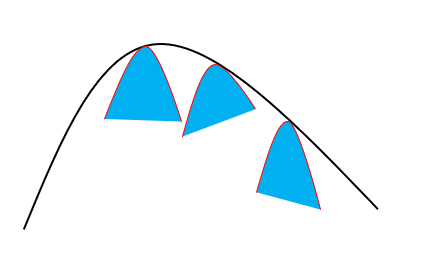
\includegraphics[width=0.5\textwidth]{TRPO.png}
\caption{The black curse is our true objective, and we optimize red lower bound in local blue region.}
\end{figure}
The original objective author consider is expected discounted reward,
\begin{equation}
    \eta(\pi) = \E_{s_0,a_0,\cdots \sim \pi}[\sum_{t=0}^{+\infty}\gamma^t r(s_t)],
\end{equation}
where the initial state $s_0 \sim \rho_0(s)$.
We can prove the difference between two policies $\pi, \tilde{\pi}$ is,
\begin{equation}
    \label{eq:TRPO_eta}
    \eta(\tilde{\pi}) = \eta(\pi) + \E_{s_0, a_0, \cdots \sim \tilde{\pi}}[\sum_{t=0}^{+\infty}\gamma^tA_{\pi}(s_t,a_t)].
\end{equation}
Intutively, it can be explained as: We have two kinds of trajectories generated by $\pi, \tilde{\pi}$, the difference is the accumulated advantage of each element in trajectory generated by $\tilde{\pi}$. Besides, we can show the simple proof. $A_{\pi}(s,a) = Q_{\pi}(s,a)-V_{\pi}(s) = \E_{s'\sim P(\cdot|s,a)}[r(s)+\gamma V_{\pi}(s')-V_{\pi}(s)]$. To simplify the notation, we use $\tau$ denote the trajectory $s_0, a_0, \cdots$.
\begin{equation}
\aligned 
\E_{\tau\sim\tilde{\pi}}\sum_{t=0}^{+\infty} \gamma^t A_{\pi}(s_t,a_t) & = \E_{\tau \sim \tilde{\pi}}\sum_{t=0}^{+\infty} \gamma^t (r(s_t)+\gamma V_{\pi}(s_{t+1}) - V_{\pi}(s_t)) \\ & = \eta(\tilde{\pi}) - \E_{s_0}[V_{\pi}(s_0)] \\ & = \eta(\tilde{\pi}) - \eta(\pi)
\endaligned
\end{equation}
Also, we can rewrite Eq.(\ref{eq:TRPO_eta}) as, 
\begin{equation}
    \label{eq: TRPO_eta1}
    \eta(\tilde{\pi}) = \eta(\pi) + \sum_{s}\rho_{\tilde{\pi}}(s)\sum_a \tilde{\pi}(s|a)A_{\pi}(s,a),
\end{equation}
where $\rho_{\tilde{\pi}}$ is discounted density of state under policy $\tilde{\pi}$. In practice, the optimization of Eq.(\ref{eq: TRPO_eta1}) has possibility making errors because of approximation error. Instead, we use another function,
\begin{equation}
    L_{\pi}(\tilde{\pi}) =\eta(\pi) + \sum_s \rho_{\pi}(s) \sum_a \tilde{\pi}(a|s)A_{\pi}(s,a).
\end{equation}
The author proved the following two theorem, which introduce two lower bounds of $L_{\pi}(\tilde{\pi})$, and then we can optimize these two lower bounds. Before statement, we give a measure of two distributions, $D_{TV}(p\|q) = \frac{1}{2}\sum_i |p_i -q_i|$. Hence, the difference between two policies can be described as, 
\begin{equation}
    D_{TV}^{\max} = \max_s D_{TV}(\pi(\cdot|s), \tilde{\pi}(\cdot|s)).
\end{equation}
\begin{theorem}
    \label{th:TRPO_lowerbound}
    Let $\alpha = D_{TV}^{\max}(\tilde{\pi},\pi)$. Then the following bound holds:
    \begin{equation}
        \eta(\tilde{\pi}) \ge L_{\pi}(\tilde{\pi}) - \frac{4\epsilon\gamma}{(1-\gamma)^2}\alpha^2, \epsilon = \max_{s,a}|A_{\pi}(s,a)|
    \end{equation}
    Besides, 
    \begin{equation}
        \eta(\tilde{\pi}) = L_{\pi}(\tilde{\pi}) - \frac{4\epsilon\gamma}{(1-\gamma)^2}D_{KL}^{\max}(\pi,\tilde{\pi}),
    \end{equation}
    where $D_{KL}$ is KL divergence.
\end{theorem}
Hence, the optimization problem can be stated as,
\begin{equation}
\max_{\theta} L_{\theta_{old}} - C D_{KL}^{\max}(\theta,\theta_{old})
\end{equation}
But if we directly take $C=\frac{4\epsilon\gamma}{(1-\gamma)^2}$ and do optimization, it can be shown that step size is too small. Hence, author modify this problem slightly: 1) give a constraint on KL divergence; 2) replace $D_{KL}^{\max}$ by an averaged KL divergence $\bar{D}_{KL}^{\rho} = \E_{s\sim \rho}[D_{KL}(\pi(\cdot|s), \tilde{\pi}(\cdot|s))]$.
\begin{equation}
\aligned 
& \max_{\theta}L_{\theta_{old}}(\theta) \\ 
& \mathrm{s.t.} \bar{D}_{KL}^{\theta_{old}}(\theta,\theta_{old}) \le \delta.
\endaligned 
\end{equation}
We can make it more practical by using importance sampling, with an off policy $q$, 
\begin{equation}
\aligned 
& \max_{\theta} \E_{s\sim \rho_{old}, a\sim q}[\frac{\pi_{\theta}(a|s)}{q(a|s)}Q_{\theta_{old}}(s,a)] \\ 
& \mathrm{s.t.} \E_{s\sim \rho_{old}}[D_{KL}(\pi_{old}(\cdot|s), \pi(\cdot|s))] \le \delta.
\endaligned
\end{equation}

%-----------------------------------------------------------------------------------------------------------------
\section{PPO}
PPO\cite{schulman2017proximal} is the simplified version of TRPO, since the latter is very computionally complex. In Policy gradient methods, the most commonly used gradient estimator has the form:
\begin{equation}
\hat{g} = \E_t[\nabla_{\theta}\pi_{\theta}(a_t|s_t)\hat{A}_t]
\end{equation}
Also, use automatic differentiation software, we can optimize the following loss function instead,
\begin{equation}
    L^{\mathrm{PG}} = \E_t[\log\pi_{\theta}(a_t|s_t)A_t].
\end{equation}
In TRPO, an objective function is maximized subject to a constraint on the size of the policy update,
\begin{equation}
\aligned 
    & \max_{\theta} \E_t[\frac{\pi_{\theta}(a_t|s_t)}{\pi_{\mathrm{old}}(a_t|s_t)}\hat{A}_t] \\ 
    & \mathrm{s.t.} \E_t[\mathrm{KL}[\pi_{\mathrm{old}}(\cdot|s_t),\pi_{\theta}(\cdot|s_t)]] \le \delta.
\endaligned 
\end{equation}
The idea in TRPO suggests using a penalty instead of a constraint, i.e solving the unconstrained optimization problem,
\begin{equation}
    \max_{\theta} \E_t[\frac{\pi_{\theta}(a_t|s_t)}{\pi_{\mathrm{old}}(a_t|s_t)} -\beta \mathrm{KL}\pi_{\mathrm{old}}(\cdot|s_t),\pi_{\theta}(\cdot|s_t)]]
\end{equation}

\subsection{clipped Surrogate Objective}
In this paper, the author raises another new objective defined as,
\begin{equation}
L^{CLIP}(\theta) = \E_t[\min(r_t(\theta)\hat{A}_t, \mathrm{clip}(r_t(\theta),1+\epsilon,1-\epsilon)\hat{A}_t)],
\end{equation}
where $r_t = \frac{\pi_{\theta}(a_t|s_t)}{\pi_{\theta_{\mathrm{old}}}(a_t|s_t)}$, and $\epsilon$ is hyperparameter, say, $\epsilon=0.2$.
And now, we can combine everything together, the final objective is,
\begin{equation}
L_{t}^{\mathrm{CLIP}+\mathrm{VF}+\mathrm{entropy}} = \E_t[L_t^{\mathrm{CLIP}}-c_1L_t^{\mathrm{VF}}(\theta)+c_2S[\pi_{\theta}](s_t)],
\end{equation}
where $c_1,c_2$ are coefficients, and $S$ denotes an entropy bonus, and $L_t^{\mathrm{VF}}$ is a squared-error loss $(V_{\theta}(s_t) - V_t^{\mathrm{target}})^2$.
\section{Asynchronous Methods for Deep Reinforcement Learning}
Deep neural networks give sufficient representations to value function and policy, but which causes training process quite
unstable. There are many approaches raised to solve this problem, and they share the same idea: the sequence of observed 
data and encounted by an online RL agents is non-stationary, and online RL updates are strongly correlated. By storing the 
agent in an experience replay memory, the data can be batched or randomly sampled from different time-steps. Aggregating over memory in this way reduces non-stationary and decorrelates updateds, but at the same time limits method to off-policy reinforment learning algorithms. In this paper, author provide a very different paradigm for deep reinforcement learning. Instead of experience replay, we asynchronously excute multiple agents in parallel, on multiple instances of environment. This parallelism also decorrelates the agents' data into a more stationary process. since at any given time-step the parallel agents will be experiencing a variety of different state.

\begin{tcolorbox}[title=A3C algorithm]
Initialise $\theta,\theta_v, T=0$.\par 
Initialise thread step $t \leftarrow 1$ \par 
Repeat:\par 
\hspace{1cm} Reset gradients: $d\theta \leftarrow 0, d\theta_v \leftarrow 0$. \par 
\hspace{1cm} Synchronize thread-specificc parameters $\theta' =\theta, \theta_v'=\theta_v$\par 
\hspace{1cm} $t_{\mathrm{start}} = t$ \par 
\hspace{1cm} Get state $s_t$ \par 
\hspace{1cm} Repeat:\par 
\hspace{2cm} Perform $a_t$ according to $\pi_{\theta}(a_t|s_t)$ \par 
\hspace{2cm} Receieve $r_t$ and new state $s_{t+1}$\par
\hspace{2cm} $t \leftarrow t+1, T \leftarrow T+1 $ \par 
\hspace{1cm} Until terminal $s_t$ or $t-t_{\mathrm{start}} == t_{\max}$ \par 
\hspace{1cm} 
\begin{equation}
    R = \left\{\begin{array}{cc}
        0, & \mathrm{for terminal state} \\ 
        V(s_t, \theta_v') & \mathrm{otherwise}
    \end{array}\right.
\end{equation}
\hspace{1cm} for $i \in \{1,2,\cdots,t_{\mathrm{start}}\}$ do\par 
\hspace{2cm} $R \leftarrow r_i + \gamma R$ \par 
\hspace{2cm} Accumlate gradient wrt $\theta'$: $d\theta \leftarrow d\theta + \nabla_{\theta'} \log \pi(a_i|s_i;\theta')(R-V(s_i;\theta_v'))$ \par 
\hspace{2cm} Accumlate gradient wrt $\theta_v'$: $d\theta_v \leftarrow d\theta_v + \nabla_{\theta_v'}(R-V(s_i;\theta_v'))^2$\par 
\hspace{1cm} end for\par 
\hspace{1cm} Perform asynchronous update $\theta$ using $d\theta$ and $\theta_v$ using $d\theta_v$. \par 
Until $T > T_{\max}$. 
\end{tcolorbox}





\clearpage
\bibliographystyle{unsrt}
\bibliography{RL}


\appendix
\section{Lists of Proofs}
\subsection{TRPO}
\subsubsection{Proof Th.\ref{th:TRPO_lowerbound}}
Defined average advantage over a different policy as,
\begin{equation}
    \bar{A}(s) = \E_{a\sim \pi(\cdot|s)}A_{\pi}(s,a)
\end{equation}
\begin{definition}[$\alpha$ coupled policy]
$(\pi,\tilde{\pi})$ is an $\alpha$ coupled policy pair if it defines a joint distribution $(a,\tilde{a})|s$, such that $P(a\neq\tilde{a}|s) \le \alpha, \forall s$. $\pi$ and $\tilde{\pi}$ denote the marginal distributions of $a$ and $\tilde{a}$, respectively.
\end{definition}
\begin{lemma}
    \label{lem: TRPO1}
    Given that $\pi, \tilde{\pi}$ are $\alpha$ coupled policies, for all $s$, 
    \begin{equation}
        |\bar{A}(s)| \le 2\alpha \max_{s,a} |A_{\pi}(s,a)|.
    \end{equation}
\end{lemma}
\emph{Proof}:
\begin{equation}
    \aligned
    |\bar{A}(s)| & = |\E_{\tilde{a}\sim\tilde{\pi}}A_{\pi}(s,\tilde{a})| \\ 
    & = |\E_{(\tilde{a},a)\sim(\tilde{\pi},\pi)}[A_{\pi}(s,\tilde(a)) - A_{\pi}(s,a)]| \\ 
    & \le 2\max_{s,a}|A_{\pi}(s,a)|.
    \endaligned
\end{equation}
\begin{lemma}
    Let $(\pi,\tilde{\pi})$ be an $\alpha$ coupled policy pair. Then,
    \begin{equation}
        |\E_{s_t\sim\tilde{\pi}}[\bar{A}(s_t)]-\E_{s_t\sim\pi}[\bar{A}(s_t)]| \le 4\alpha(1-(1-\alpha)^t) \max_{s,a} |A_{\pi}(s,a)|.
    \end{equation}
\end{lemma}
\emph{Proof}:
The expectation difference is caused by each sampled state $s_i, i< t$, which is different between two trajectories generated by $\tilde{\pi}$ and $\pi$. Hence, we can introduce random variable $n_t$ denote the different state number up to time $t$. Then, 
\begin{equation}
    |\E_{s_t\sim\tilde{\pi}}[\bar{A}(s_t)]-\E_{s_t\sim\pi}[\bar{A}(s_t)]| = P(n_t>0)|\E_{s_t\sim\tilde{\pi}|n_t>0}[\bar{A}(s_t)]-\E_{s_t\sim\pi|n_t>0}[\bar{A}(s_t)]|.
\end{equation}
Since each step, the different probability is samller than $\alpha$, then $P(n_t>0) \le 1 - (1-\alpha)^t$. And the second part is not greater than $4\alpha \max_{s,a}|A_{\pi}(s,a)|$ from Lemma.(\ref{lem: TRPO1}).
QED.\\ 
\emph{Proof of Theorem}:
Use $\epsilon = \max_{s,a}|A_{\pi}(s,a)|$
\begin{equation}
\aligned 
\eta(\tilde{\pi}) - L_{\pi}(\tilde{\pi}) & = \sum_{t=0}^{+\infty} \gamma^t |\E_{\tau|\tilde{\pi}}\bar{A}(s_t) - \E_{\tau|\pi}\bar{A}(s_t)| \\ 
& \le \sum_{t=0}^{t=\infty} \gamma^t 4\alpha \epsilon (1-(1-\alpha)^t) \\ 
& \le \frac{4\alpha^2\gamma \epsilon}{(1-\gamma)^2}
\endaligned
\end{equation}
Obivously, if we take $\alpha = D_{TV}^{\max}$, everything keeps invariant.























\end{document}